%----------------------------------------------------------------------------------------
% EERSTEGRAADSFUNCTIES. Alle opgaven zijn eigen werk.
%
% Opbouw: Probleem, Start, leerstof, en op een nieuwe pagina de Opdrachten en Test jezelf (geen Koppel in de 2de graad).
% Labels van dit hoofdstuk beginnen met h2-.
% Notatie: rico m en voorschrift f(x) = mx + q (zoals m = 1/6 op de voorkant).
% Verschillen per pakket: de vorm y - y1 = m(x - x1) (4-5), het bewijs bij de stappen in een tabel (5),
% en in de oefeningenbank een opdracht met de puntrichtingsvorm (4-5) en een bewijsopdracht (5).
%----------------------------------------------------------------------------------------

\mychapter{2}{Eerstegraadsfuncties}

\begin{probleem}
\vspace{-1mm}\naast{Een podium in de turnzaal is 50 cm hoog. Om er met een rolstoel op te rijden, komt er een oprit: een rechte plank van de vloer tot op het podium. Oprit A begint 3 m voor het podium, oprit B al 2,4 m ervoor (horizontaal gemeten). Welke oprit is het steilst, en hoeveel steiler? Hoe hoog ben je op oprit A als je 1,2 m ver bent? En volgend jaar komt er een podium van 80 cm: hoe ver voor dat podium moet een oprit beginnen die even steil is als A?}{\begin{tikzpicture}[x=1.45cm,y=1.45cm,font=\scriptsize]
  \fill[accent!20] (3,0) rectangle (3.7,.5);
  \draw[accent] (3,0) rectangle (3.7,.5);
  \node at (3.35,.25) {podium};
  \draw[accent,very thick] (0,0) -- (3,.5);
  \draw[inkt,thick,dashed] (.6,0) -- (3,.5);
  \draw[grijs] (-.15,0) -- (3.9,0);
  \node[above,text=accent] at (1.2,.22) {A};
  \node[below,text=inkt] at (1.9,.25) {B};
  \draw[grijs,<->] (3.82,0) -- (3.82,.5) node[midway,right] {$0,5$ m};
  \draw[grijs,<->] (0,-.18) -- (3,-.18) node[midway,below] {$3$ m};
  \draw[grijs,<->] (.6,-.48) -- (3,-.48) node[midway,below] {$2,4$ m};
\end{tikzpicture}}
\end{probleem}

\lkr{Leerplan \pakketnaam: LPD \alleenvoor{1,2,3}{17-21}\alleenvoor{4,5}{21-25} (dit hoofdstuk: rechte evenredigheid, de richtingscoëfficiënt, de eerstegraadsfunctie in voorschrift, tabel en grafiek, het voorschrift opstellen\alleenvoor{4,5}{ (ook met de vorm $y - y_1 = m(x - x_1)$)} en eerstegraadsmodellen in een context). Welke nummers precies bij dit hoofdstuk horen, is na te kijken in het leerplan. Voorkennis: hoofdstuk 1 en eerstegraadsvergelijkingen oplossen; dat laatste wordt kort herhaald waar het nodig is. Notatie: de rico heet $m$ en het voorschrift $f(x) = mx + q$, zoals $m = \tfrac16$ op de voorkant. Gebruikt uw school $f(x) = ax + b$, vermeld dat dan in de les. Laat de leerlingen het probleem eerst proberen: de meesten voelen aan dat B steiler is, maar ``hoeveel steiler'' vraagt een getal.}

Sommige verbanden zijn heel eenvoudig: elke minuut loopt er evenveel water uit een ton, elke kilometer met de taxi kost evenveel extra. Hun grafiek is een rechte. In dit hoofdstuk leer je hoe steil zo'n rechte is: dat zegt één getal, de \textit{richtingscoëfficiënt}. Met dat getal en het punt waar de rechte de $y$-as snijdt, schrijf je het voorschrift, teken je de grafiek en vul je een tabel aan. Op het einde kun je het voorschrift opstellen bij een grafiek, bij twee punten en bij een situatie uit het dagelijks leven.

\begin{oefeningen}[Start]
\oef{h2-start-1}

\oef{h2-verken}
\end{oefeningen}

%========================================================================================
\section{Rechte evenredigheid}

Oprit A stijgt gelijkmatig. Meet op een horizontale afstand $x$ van het begin hoe hoog de plank is: dat is de hoogte $h$, allebei in meter. Op 3 m ben je op het podium, op 0,5 m hoogte. Halverwege, op 1,5 m, ben je halverwege de hoogte: 0,25 m. Zo krijg je deze tabel.

\naast{\waardetabel[$x$ (m)][$h$ (m)]{6}{0 & 0,6 & 1,2 & 1,8 & 2,4 & 3}{0 & 0,1 & 0,2 & 0,3 & 0,4 & 0,5}

\vspace{2mm}
Wat valt op? Verdubbel je $x$, dan verdubbelt ook $h$: van 0,6 naar 1,2 m gaat de hoogte van 0,1 naar 0,2 m. De punten van de tabel liggen op een rechte door de oorsprong. (In de figuur is de hoogte drie keer vergroot, anders zie je de helling bijna niet.)}{\begin{tikzpicture}[x=1.05cm,y=3.15cm]
  \roosterleeg[$x$][$h$]{0}{0.6}{3.6}{0}{0.1}{0.6}
  \xlabels{1.2/{1,2},2.4/{2,4},3.6/{3,6}}
  \ylabels{0.2/{0,2},0.4/{0,4},0.6/{0,6}}
  \oorsprong
  \rechte{0}{3.6}{1/6}{0}
  \foreach \t in {0,0.6,1.2,1.8,2.4,3}{\punt{\t}{\t/6}}
\end{tikzpicture}}

Deel je $h$ door $x$, dan krijg je telkens hetzelfde getal:
\[\frac{0,1}{0,6} = \frac{0,2}{1,2} = \frac{0,3}{1,8} = \frac{0,4}{2,4} = \frac{0,5}{3} = \frac16.\]
De hoogte is dus altijd $\tfrac16$ van de afstand: $h = \tfrac16\,x$.

\begin{theorie}
Twee grootheden $x$ en $y$ zijn \textbf{\textcolor{accent}{recht evenredig}} als het quotiënt $\tfrac yx$ voor elke $x \neq 0$ hetzelfde getal $m$ is, met $m \neq 0$. Dan is

\vspace{1mm}
\qquad $\formule{y = m\,x}$
\end{theorie}

Het getal $m$ heet de \textit{evenredigheidsfactor}. Bij oprit A is $m = \tfrac16$. Waarom gaat de grafiek door de oorsprong? Voor $x = 0$ is $y = m \cdot 0 = 0$. In de volgende sectie zien we dat $m$ ook zegt hoe steil de rechte is.

\voorbeeld{}{Bij een tankstation betaal je voor $x$ liter benzine $p$ euro. Zijn $x$ en $p$ recht evenredig? Zo ja, geef het voorschrift.

\vspace{1mm}
\waardetabel[$x$ (l)][$p$ (euro)]{4}{5 & 10 & 25 & 40}{9 & 18 & 45 & 72}\label{vb:h2-evenredig}}{%
\uitleg{We delen in elke kolom $p$ door $x$. Is het quotiënt altijd hetzelfde, dan zijn de grootheden recht evenredig.}
\begin{stappen}
\frac95 = \frac{18}{10} = \frac{45}{25} = \frac{72}{40} = 1,8 & Het quotiënt is telkens 1,8: recht evenredig. \\
p = 1,8\,x & De evenredigheidsfactor is de prijs van 1 liter: 1,80 euro.
\end{stappen}}

\voorbeeld{}{Een taxirit kost $k$ euro voor $x$ km. Zijn $x$ en $k$ recht evenredig?

\vspace{1mm}
\waardetabel[$x$ (km)][$k$ (euro)]{3}{2 & 5 & 10}{7 & 13 & 23}\label{vb:h2-nietevenredig}}{%
\uitleg{Ook hier delen we $k$ door $x$, en kijken of het quotiënt gelijk blijft.}
\begin{stappen}
\frac72 = 3,5 \qquad \frac{13}{5} = 2,6 \qquad \frac{23}{10} = 2,3 & De quotiënten verschillen: niet recht evenredig.
\end{stappen}
Een rit van 10 km kost ook niet het dubbele van een rit van 5 km. Toch is het een eenvoudig verband: elke kilometer extra kost $\tfrac{13 - 7}{5 - 2} = 2$ euro. Daar komen we verderop in dit hoofdstuk op terug.}

\begin{werkwijze}
Deel in elke kolom van de tabel $y$ door $x$. Is het quotiënt overal hetzelfde getal $m$, dan zijn $x$ en $y$ recht evenredig, met voorschrift $y = mx$. Is één quotiënt anders, dan niet.
\end{werkwijze}

\begin{oefeningen}
\oef{h2-evenredig}
\end{oefeningen}

%========================================================================================
\section{De richtingscoëfficiënt}

\subsection{Hoe steil is een rechte?}

Oprit A en oprit B zijn allebei rechte planken, maar B is steiler. Hoe druk je met een getal uit hoe steil een rechte is? Kijk naar een trapje onder de rechte: ga een stuk opzij, en meet hoeveel je moet stijgen om weer op de rechte te komen. Bij oprit A stijg je 0,1 m als je 0,6 m opzij gaat. Verleng je de plank in gedachten, dan stijg je 1 m als je 6 m opzij gaat, zoals op de voorkant van dit boek. Een klein of een groot trapje: de verhouding is dezelfde, $\tfrac{1}{6} = \tfrac{0,5}{3} = \tfrac{0,1}{0,6}$. Dat getal meet hoe steil de rechte is. De figuur toont twee trapjes onder een rechte die even steil is als oprit A.

\figuren{\begin{tikzpicture}[x=.72cm,y=.72cm]
  \roosterleeg{0}{1}{12}{0}{1}{3}
  \xgetallen{2,4,6,8,10,12}\ygetallen{1,2,3}\oorsprong
  \rechte{0}{12}{1/6}{1}
  \trapje{0}{1}{6}{1}{$6$ opzij}{$1$ omhoog}
  \trapje{9}{2.5}{3}{0.5}{$3$ opzij}{$\tfrac12$ omhoog}
  \punt{0}{1}\punt{6}{2}\punt{9}{2.5}\punt{12}{3}
  \node[accent,above left,font=\footnotesize] at (4,1.67) {rico $\tfrac16$};
\end{tikzpicture}}

Het getal hangt dus niet af van het trapje dat je kiest: een groter trapje is een vergroting van een kleiner, met dezelfde vorm. Gaat de rechte door twee punten $(x_1, y_1)$ en $(x_2, y_2)$, dan ga je $x_2 - x_1$ opzij en $y_2 - y_1$ omhoog.

\begin{theorie}
De \textbf{\textcolor{accent}{richtingscoëfficiënt}} (kort: \textbf{\textcolor{accent}{rico}}) van een rechte door twee punten $(x_1, y_1)$ en $(x_2, y_2)$ met $x_1 \neq x_2$ is

\vspace{1mm}
\qquad $\formule{m = \dfrac{y_2 - y_1}{x_2 - x_1}}$ \qquad $= \dfrac{\text{verandering van } y}{\text{verandering van } x}$
\end{theorie}

De volgorde van de punten mag je kiezen, als je ze maar in de teller en de noemer gelijk houdt: begin je boven met $y_2$, dan begin je onder met $x_2$. Gaat de rechte naar beneden, dan is $y_2 - y_1$ negatief en daalt het trapje: de rico is negatief.

\voorbeeld{}{Bereken de rico van de rechte door $A(-1, 4)$ en $B(3, -2)$.\label{vb:h2-rico}}{%
\naast{\uitleg{We vullen de formule in met $A$ als eerste punt en $B$ als tweede, en controleren met een trapje.}
\begin{stappenvrij}{4.4cm}{4.6cm}
m = \frac{-2 - 4}{3 - (-1)} & Verandering van $y$ gedeeld door verandering van $x$. \\
= \frac{-6}{4} = -\frac32 & Vereenvoudig de breuk.
\end{stappenvrij}
\vspace{1mm}
Het trapje gaat 4 opzij en 6 omlaag. De rico is negatief: de rechte daalt.}{\begin{tikzpicture}[x=.45cm,y=.45cm]
  \rooster{-2}{1}{4}{-3}{1}{5}
  \rechte{-2}{3.6}{-3/2}{2.5}
  \trapje{-1}{4}{4}{-6}{$4$}{$-6$}
  \punt{-1}{4}\punt{3}{-2}
  \node[left,font=\scriptsize] at (-1,4) {$A$};
  \node[left,font=\scriptsize] at (3,-2) {$B$};
\end{tikzpicture}}}

\nujij{Bereken de rico van de rechte door $(2, 1)$ en $(6, 3)$.}{$m = \tfrac{3 - 1}{6 - 2} = \tfrac24 = \tfrac12$.}

\begin{oefeningen}
\oef{h2-rico}
\end{oefeningen}

\subsection{Stijgen, dalen en steilheid}

Wat vertelt het teken van de rico? De figuur toont rechten door de oorsprong, met hun rico erbij. Is $m$ positief, dan stijgt de rechte van links naar rechts. Is $m$ negatief, dan daalt ze. Bij $m = 0$ ga je opzij zonder te stijgen: de rechte is horizontaal. En hoe groter $\abs{m}$, de rico zonder zijn teken, hoe steiler de rechte: $m = 2$ en $m = -2$ zijn even steil, de ene stijgt en de andere daalt.

\naast{\begin{stappenvrij}{3.3cm}{5.6cm}
m > 0 & de rechte stijgt \\
m < 0 & de rechte daalt \\
m = 0 & de rechte is horizontaal \\
\abs{m} \text{ groter} & de rechte is steiler
\end{stappenvrij}

\vspace{2mm}
Een verticale rechte heeft geen rico: twee punten erop hebben dezelfde $x$, en dan deel je door $x_2 - x_1 = 0$.}{\begin{tikzpicture}[x=.5cm,y=.5cm,font=\scriptsize]
  \rooster{-3}{1}{3}{-3}{1}{3}
  \foreach \m/\e in {2/1.5,1/3,0.5/3,0/3,-0.5/3,-2/1.5}{\rechte{-\e}{\e}{\m}{0}}
  \node[above] at (1.5,3) {$2$};
  \node[right] at (3,3) {$1$};
  \node[right] at (3,1.5) {$\tfrac12$};
  \node[right] at (3,0.3) {$0$};
  \node[right] at (3,-1.5) {$-\tfrac12$};
  \node[below] at (1.5,-3) {$-2$};
\end{tikzpicture}}

Op een rooster lees je de rico af met een trapje: zoek twee punten van de rechte op de kruispunten van het rooster, en tel de hokjes.

\voorbeeld{}{Lees de rico af van de rechte in de figuur.\label{vb:h2-ricografiek}}{%
\naast{\uitleg{We zoeken twee punten van de rechte die precies op een kruispunt van het rooster liggen, en tekenen er een trapje tussen.}
\begin{stappenvrij}{3.6cm}{5.4cm}
(-2, -1) \text{ en } (2, 2) & Twee kruispunten op de rechte. \\
4 \text{ opzij}, \ 3 \text{ omhoog} & Tel de hokjes van het trapje. \\
m = \frac34 & Omhoog gedeeld door opzij.
\end{stappenvrij}}{\begin{tikzpicture}[x=.45cm,y=.45cm]
  \rooster{-3}{1}{4}{-3}{1}{3}
  \rechte{-3}{3.5}{3/4}{0.5}
  \trapje{-2}{-1}{4}{3}{$4$}{$3$}
  \punt{-2}{-1}\punt{2}{2}
\end{tikzpicture}}}

\begin{werkwijze}
Ken je twee punten, deel dan de verandering van $y$ door de verandering van $x$, in dezelfde volgorde. Lees je af op een grafiek, kies dan twee punten op kruispunten van het rooster en teken een trapje: de rico is omhoog gedeeld door opzij, met een minteken als je omlaag gaat.
\end{werkwijze}

\begin{oefeningen}
\oef{h2-rico-grafiek}
\end{oefeningen}

Nu kunnen we de vragen van het probleem beantwoorden.

\voorbeeld{}{Terug naar het probleem. Welke oprit is het steilst, en hoeveel? Hoe hoog ben je op oprit A na 1,2 m? Hoe ver voor een podium van 80 cm begint een oprit die even steil is als A?\label{vb:h2-terug}}{%
\uitleg{De steilheid van een oprit is zijn rico: de hoogte gedeeld door de horizontale afstand. Bij oprit A hoort de rechte evenredigheid $h = \tfrac16 x$ uit de eerste sectie.}
\begin{stappenbreed}
m_A = \frac{0,5}{3} = \frac16 \approx 0,17 \qquad m_B = \frac{0,5}{2,4} = \frac{5}{24} \approx 0,21 & Oprit A stijgt 1 m per 6 m, B ongeveer 0,21 m per meter. \\
\frac{m_B}{m_A} = \frac{5}{24} \cdot 6 = \frac54 = 1,25 & B is $1,25$ keer zo steil als A. \\
h = \frac16 \cdot 1,2 = 0,2 & Na 1,2 m ben je 0,2 m hoog. \\
0,8 = \frac16\,x \quad\Longrightarrow\quad x = 6 \cdot 0,8 = 4,8 & Even steil: dezelfde rico $\tfrac16$.
\end{stappenbreed}
Oprit B is het steilst: een kwart steiler dan A. Op oprit A ben je na 1,2 m op 20 cm hoogte. Voor een podium van 80 cm moet de oprit 4,8 m voor het podium beginnen. Elke oprit met rico $\tfrac16$ heeft zo'n trapje: 6 opzij, 1 omhoog.}

%========================================================================================
\section{De eerstegraadsfunctie}

\subsection{Een rechte die niet door de oorsprong gaat}

Terug naar de taxi uit voorbeeld~\ref{vb:h2-nietevenredig}. Zodra je instapt, betaal je al 3 euro. Daarna kost elke kilometer 2 euro. Voor $x$ km betaal je dus $k(x) = 2x + 3$ euro. Dat verband is niet recht evenredig, want voor 0 km betaal je al 3 euro. Maar de grafiek is wel een rechte: elke kilometer komt er 2 euro bij, dus elk trapje van 1 opzij gaat 2 omhoog. De rico is 2, en de rechte snijdt de $y$-as in $(0, 3)$.

\naast{\waardetabel[$x$ (km)][$k(x)$ (euro)]{5}{0 & 1 & 2 & 3 & 4}{3 & 5 & 7 & 9 & 11}

\vspace{2mm}
In de tabel zie je de rico terug: telkens als $x$ met 1 toeneemt, neemt $k(x)$ met 2 toe. Het getal 3 is de \textit{beginwaarde}: de prijs voor 0 km. Zo'n voorschrift, met $x$ tot de eerste macht, heet een eerstegraadsfunctie.}{\begin{tikzpicture}[x=.6cm,y=.24cm]
  \roosterleeg[$x$][$k$]{0}{1}{5}{0}{2}{13}
  \xgetallen{1,2,3,4,5}\ygetallen{2,4,6,8,10,12}\oorsprong
  \rechte{0}{5}{2}{3}
  \trapje{1}{5}{1}{2}{$1$}{$2$}
  \foreach \t in {0,...,4}{\punt{\t}{2*\t+3}}
\end{tikzpicture}}

\begin{theorie}
Een \textbf{\textcolor{accent}{eerstegraadsfunctie}} is een functie met een voorschrift van de vorm

\vspace{1mm}
\qquad $\formule{f(x) = mx + q}$ \qquad met $m$ en $q$ reële getallen en $m \neq 0$.

\vspace{1mm}
Haar grafiek is een rechte met rico $m$ die de $y$-as snijdt in het punt $\formule{(0, q)}$.
\end{theorie}

Waarom is $(0, q)$ het snijpunt met de $y$-as? Op de $y$-as is $x = 0$, en $f(0) = m \cdot 0 + q = q$. In een context is $q$ vaak de beginwaarde, zoals de instapprijs van de taxi. Twee bijzondere gevallen ken je al of zie je nu:
\begin{itemize}
\item Is $q = 0$, dan is $f(x) = mx$: een rechte evenredigheid, met een grafiek door de oorsprong.
\item Is $m = 0$, dan is $f(x) = q$ voor elke $x$. Dat is geen eerstegraadsfunctie meer, maar een \textit{constante functie}. Haar grafiek is een horizontale rechte.
\end{itemize}

\voorbeeld{}{Geef de rico en het snijpunt met de $y$-as van de grafiek van $f(x) = 5 - 2x$. Stijgt of daalt de grafiek?\label{vb:h2-mq}}{%
\uitleg{Het voorschrift staat niet in de volgorde $mx + q$. We wisselen de termen, met hun teken.}
\begin{stappen}
f(x) = -2x + 5 & De term met $x$ vooraan; het minteken hoort bij $2x$. \\
m = -2, \quad q = 5 & De rico is de coëfficiënt van $x$. \\
(0, 5) & Het snijpunt met de $y$-as. \\
m < 0 & De grafiek daalt.
\end{stappen}
Let op bij een voorschrift met haakjes, zoals $g(x) = 3(x - 1)$: werk eerst de haakjes uit, $g(x) = 3x - 3$. Dan is $m = 3$ en $q = -3$, en niet $-1$.}

\subsection{De grafiek tekenen}

Om een rechte te tekenen, heb je twee punten nodig. Met $m$ en $q$ vind je ze zonder te rekenen: begin op de $y$-as in $(0, q)$, en zet vanaf daar een trapje met de rico.

\voorbeeld{}{Teken de grafiek van $f(x) = \tfrac23 x - 1$.\label{vb:h2-tekenen}}{%
\naast{\uitleg{We beginnen in het snijpunt met de $y$-as. De rico $\tfrac23$ lezen we als 3 opzij en 2 omhoog.}
\begin{stappenvrij}{3cm}{6cm}
(0, -1) & Het snijpunt met de $y$-as, want $q = -1$. \\
(3, 1) & 3 opzij en 2 omhoog. \\
(6, 3) & Nog een trapje: ter controle. \\
f(-3) = -3 & Controle met het voorschrift: $(-3, -3)$ ligt op de rechte.
\end{stappenvrij}}{\begin{tikzpicture}[x=.42cm,y=.42cm]
  \rooster{-4}{1}{7}{-4}{1}{4}
  \rechte{-4}{7}{2/3}{-1}
  \trapje{0}{-1}{3}{2}{$3$}{$2$}
  \trapje{3}{1}{3}{2}{$3$}{$2$}
  \punt{0}{-1}\punt{3}{1}\punt{6}{3}\punt{-3}{-3}
\end{tikzpicture}}}

Is de rico negatief, dan gaat het trapje omlaag: bij $m = -\tfrac23$ ga je 3 opzij en 2 omlaag. Is de rico een geheel getal, zoals $m = -2$, lees het dan als $\tfrac{-2}{1}$: 1 opzij en 2 omlaag.

\begin{werkwijze}
Zet het punt $(0, q)$ op de $y$-as. Schrijf de rico als breuk $\tfrac{\text{omhoog}}{\text{opzij}}$, en zet vanaf $(0, q)$ een trapje: zoveel opzij, zoveel omhoog (of omlaag bij een negatieve rico). Teken de rechte door de punten, en controleer een punt met het voorschrift.
\end{werkwijze}

\nujij{Teken de grafiek van $g(x) = -\tfrac12 x + 2$. Door welk punt op de $x$-as gaat ze?}{Begin in $(0, 2)$, ga 2 opzij en 1 omlaag: $(2, 1)$, en nog eens: $(4, 0)$. De rechte snijdt de $x$-as in $(4, 0)$.}

\begin{oefeningen}
\oef{h2-tekenen}
\end{oefeningen}

\subsection{De tabel van een eerstegraadsfunctie}

In de tabel van de taxi steeg $k(x)$ telkens met 2 als $x$ met 1 toenam. Is dat bij elke eerstegraadsfunctie zo, ook met grotere stappen? Neem $f(x) = 3x + 1$. Van $x = 2$ naar $x = 5$ ga je 3 opzij, en $f(x)$ gaat van 7 naar 16: dat is $9 = 3 \cdot 3$ omhoog. Bij elke stap opzij komt er de rico maal die stap bij.

\begin{theorie}
\begin{stelling}{Stappen in een tabel}
Neemt bij een eerstegraadsfunctie $f(x) = mx + q$ de waarde van $x$ toe met een getal $d$, dan neemt $f(x)$ toe met

\vspace{1mm}
\qquad $\formule{m \cdot d}$

\vspace{1mm}
Bij gelijke stappen in $x$ zijn de stappen in $f(x)$ dus ook gelijk. Bij een stap 1 in $x$ neemt $f(x)$ toe met $m$.
\end{stelling}
\begin{alleenvoor}{5}
\begin{bewijs}
Neem een getal $x$ en een stap $d$. Dan is
\bewijsregel{f(x + d) - f(x) = m(x + d) + q - (mx + q) = mx + md + q - mx - q = m\,d.}
De verandering van $f(x)$ gedeeld door de verandering van $x$ is dus $\tfrac{md}{d} = m$, voor elke twee punten van de grafiek. Overal op de grafiek hoort bij een trapje dezelfde rico $m$: de grafiek is een rechte met rico $m$.
\end{bewijs}
\end{alleenvoor}
\end{theorie}

\begin{alleenvoor}{1,2,3,4}
Waarom? Ga van $x$ naar $x + d$. De term $q$ blijft gelijk, en de term $mx$ wordt $m(x + d) = mx + md$: er komt precies $md$ bij. Dat geldt voor elke twee punten van de grafiek, en daarom is de grafiek een rechte met rico $m$.
\end{alleenvoor}

Omgekeerd herken je zo een eerstegraadsfunctie in een tabel: bij gelijke stappen in $x$ moeten de stappen in $y$ gelijk zijn. Bij $x = 0, 1, 2, 3$ en $y = 1, 2, 4, 8$ zijn de stappen in $y$ eerst 1, dan 2, dan 4: dat is geen eerstegraadsfunctie.

\voorbeeld{}{Hoort deze tabel bij een eerstegraadsfunctie? Zo ja, geef het voorschrift.

\vspace{1mm}
\waardetabel{5}{-2 & 0 & 2 & 4 & 6}{9 & 6 & 3 & 0 & -3}\label{vb:h2-tabel}}{%
\uitleg{De stappen in $x$ zijn gelijk, telkens 2. We kijken of ook de stappen in $y$ gelijk zijn.}
\begin{stappen}
9 \to 6 \to 3 \to 0 \to -3 & Telkens 3 omlaag: gelijke stappen, dus een eerstegraadsfunctie. \\
m = \frac{-3}{2} = -\frac32 & De verandering van $y$ gedeeld door de stap in $x$. \\
q = f(0) = 6 & De waarde bij $x = 0$ staat in de tabel. \\
f(x) = -\tfrac32 x + 6 & Controle: $f(4) = -6 + 6 = 0$.
\end{stappen}}

\begin{oefeningen}
\oef{h2-tabel}
\end{oefeningen}

%========================================================================================
\section{Het voorschrift opstellen}

Vaak ken je het voorschrift niet, maar wel een grafiek, twee punten of een situatie. Hoe vind je dan het voorschrift? Omdat het van de vorm $f(x) = mx + q$ is, volstaat het om twee getallen te vinden: de rico $m$ en het getal $q$.

\subsection{Uit de grafiek}

Op een grafiek lees je $q$ af waar de rechte de $y$-as snijdt, en $m$ met een trapje.

\voorbeeld{}{Geef het voorschrift van de rechte in de figuur.\label{vb:h2-vgrafiek}}{%
\naast{\uitleg{We lezen eerst het snijpunt met de $y$-as af, en daarna de rico met een trapje naar een ander kruispunt van het rooster.}
\begin{stappenvrij}{3.4cm}{5.4cm}
q = 3 & De rechte snijdt de $y$-as in $(0, 3)$. \\
m = \frac{-3}{4} = -\frac34 & Van $(0, 3)$ naar $(4, 0)$: 4 opzij, 3 omlaag. \\
f(x) = -\tfrac34 x + 3 & Vul $m$ en $q$ in.
\end{stappenvrij}}{\begin{tikzpicture}[x=.45cm,y=.45cm]
  \rooster{-2}{1}{6}{-2}{1}{4}
  \rechte{-1.3}{6}{-3/4}{3}
  \trapje{0}{3}{4}{-3}{$4$}{$-3$}
  \punt{0}{3}\punt{4}{0}
\end{tikzpicture}}}

\begin{oefeningen}
\oef{h2-vgrafiek}
\end{oefeningen}

\subsection{Door twee punten}

Liggen de punten niet op de $y$-as, dan lees je $q$ niet zomaar af. De rico vind je wel met de formule. Daarna weet je: elk punt van de rechte voldoet aan $y = mx + q$. Vul je de coördinaten van een gekend punt in, dan blijft er een vergelijking over met als enige onbekende $q$. Zo'n eerstegraadsvergelijking los je op door de termen zonder $q$ naar het andere lid te brengen, met het omgekeerde teken.

\voorbeeld{}{Geef het voorschrift van de rechte door $A(2, 5)$ en $B(6, 3)$.\label{vb:h2-tweepunten}}{%
\naast{\uitleg{Eerst de rico, dan vullen we het punt $A$ in om $q$ te vinden. Met $B$ controleren we.}
\begin{stappenvrij}{4.2cm}{4.6cm}
m = \frac{3 - 5}{6 - 2} = \frac{-2}{4} = -\frac12 & De formule voor de rico. \\
5 = -\tfrac12 \cdot 2 + q & $A(2, 5)$ ligt op $y = -\tfrac12 x + q$. \\
5 = -1 + q & Reken het product uit. \\
q = 6 & Breng $-1$ naar het linkerlid: $5 + 1$. \\
y = -\tfrac12 x + 6 & Controle met $B$: $-3 + 6 = 3$.
\end{stappenvrij}}{\begin{tikzpicture}[x=.42cm,y=.42cm]
  \rooster{-1}{1}{8}{-1}{1}{7}
  \rechte{-1}{8}{-1/2}{6}
  \trapje{2}{5}{4}{-2}{$4$}{$-2$}
  \punt{2}{5}\punt{6}{3}\punt[inkt]{0}{6}
  \node[above right,font=\scriptsize] at (2,5) {$A$};
  \node[below left,font=\scriptsize] at (6,3) {$B$};
\end{tikzpicture}}}

\begin{werkwijze}
Bereken de rico met de twee punten. Vul daarna in $y = mx + q$ de rico en de coördinaten van een van de punten in, en los de vergelijking op naar $q$. Schrijf het voorschrift, en controleer met het andere punt.
\end{werkwijze}

\nujij{Geef het voorschrift van de rechte door $(1, 1)$ en $(3, 7)$.}{$m = \tfrac{7 - 1}{3 - 1} = 3$, en $1 = 3 \cdot 1 + q$ geeft $q = -2$: $y = 3x - 2$.}

\begin{oefeningen}
\oef{h2-tweepunten}
\end{oefeningen}

\begin{alleenvoor}{4,5}
\subsection{Met een punt en de rico}

Kan het ook in één keer, zonder eerst $q$ te zoeken? Neem een rechte met rico $m$ door een gekend punt $(x_1, y_1)$, en een willekeurig ander punt $(x, y)$ op die rechte. De rico tussen die twee punten is $m$:
\[\frac{y - y_1}{x - x_1} = m, \qquad\text{dus}\qquad y - y_1 = m(x - x_1).\]
Dat is een vergelijking die alle punten van de rechte beschrijft, ook het punt $(x_1, y_1)$ zelf.

\begin{theorie}
De rechte met rico $m$ door het punt $(x_1, y_1)$ heeft als vergelijking

\vspace{1mm}
\qquad $\formule{y - y_1 = m(x - x_1)}$
\end{theorie}

\voorbeeld{}{Geef het voorschrift van de rechte met rico $-\tfrac12$ door $A(2, 5)$.\label{vb:h2-puntrico}}{%
\uitleg{We vullen de rico en het punt in de vergelijking in, en werken uit tot de vorm $y = mx + q$.}
\begin{stappen}
y - 5 = -\tfrac12 (x - 2) & $m = -\tfrac12$, $x_1 = 2$ en $y_1 = 5$. \\
y - 5 = -\tfrac12 x + 1 & Werk de haakjes uit. \\
y = -\tfrac12 x + 6 & Breng $-5$ naar het rechterlid.
\end{stappen}
Dat is dezelfde rechte als in voorbeeld~\ref{vb:h2-tweepunten}: beide methodes geven hetzelfde. Ken je twee punten, bereken dan eerst de rico en kies een van de punten als $(x_1, y_1)$.}

\begin{oefeningen}
\oef{h2-puntrico}
\end{oefeningen}
\end{alleenvoor}

\subsection{In een context}

Een eerstegraadsfunctie is een goed model als een grootheid gelijkmatig verandert: elke minuut, elke kilometer of elke graad evenveel. De rico is dan de verandering per eenheid, en $q$ de waarde bij 0. Ken je twee meetwaarden, dan gebruik je ze als twee punten.

\voorbeeld{}{In de Verenigde Staten meten ze de temperatuur in graden Fahrenheit ($^\circ$F). Water bevriest bij $0\,^\circ$C of $32\,^\circ$F, en kookt bij $100\,^\circ$C of $212\,^\circ$F. Het verband is een eerstegraadsfunctie. Geef het voorschrift van $F$ in functie van $C$. Is $37\,^\circ$C koorts als je het in $^\circ$F uitdrukt? Wat betekent de rico?\label{vb:h2-context}}{%
\naast{\uitleg{De twee meetwaarden zijn twee punten: $(0, 32)$ en $(100, 212)$. Het eerste ligt op de $y$-as, dus $q$ lezen we meteen af.}
\begin{stappenvrij}{5cm}{4.6cm}
m = \frac{212 - 32}{100 - 0} = \frac{180}{100} = 1,8 & De rico. \\
q = 32 & Bij $C = 0$ is $F = 32$. \\
F = 1,8\,C + 32 & Het voorschrift. \\
1,8 \cdot 37 + 32 = 98,6 & De lichaamstemperatuur in $^\circ$F.
\end{stappenvrij}
\vspace{1mm}
De rico zegt: per graad Celsius stijgt de temperatuur met 1,8 graden Fahrenheit. Een gezond lichaam van $37\,^\circ$C is $98,6\,^\circ$F: geen koorts, ook al lijkt het getal hoog.}{\begin{tikzpicture}[x=.034cm,y=.015cm]
  \roosterleeg[$C$][$F$]{0}{20}{100}{0}{40}{240}
  \xgetallen{20,40,60,80,100}\ygetallen{40,80,120,160,200,240}\oorsprong
  \rechte{0}{100}{1.8}{32}
  \punt{0}{32}\punt{100}{212}\punt{37}{98.6}
  \aflezen{37}{98.6}
\end{tikzpicture}}}

\begin{werkwijze}
Zoek in de tekst de verandering per eenheid (de rico) en de waarde bij 0 (het getal $q$). Staan er twee meetwaarden, schrijf ze dan als punten $(x, y)$ en stel het voorschrift op door twee punten. Zeg in woorden wat $m$ en $q$ betekenen, met de eenheden.
\end{werkwijze}

\begin{oefeningen}
\oef{h2-context}
\end{oefeningen}

\subsection{Evenwijdige rechten}

Hoe zie je aan het voorschrift dat twee rechten evenwijdig zijn?

\naast{De figuur toont drie rechten met dezelfde rico $\tfrac12$. Ze zijn evenwijdig: bij elk trapje van 2 opzij gaan ze alle drie 1 omhoog, dus ze komen nooit dichter bij elkaar. Alleen het snijpunt met de $y$-as verschilt.

\vspace{1mm}
Omgekeerd hebben evenwijdige rechten dezelfde steilheid, dus dezelfde rico. Twee rechten met een verschillende rico snijden elkaar ergens.}{\begin{tikzpicture}[x=.4cm,y=.4cm,font=\scriptsize]
  \rooster{-4}{1}{4}{-4}{1}{5}
  \rechte{-4}{4}{1/2}{3}
  \rechte{-4}{4}{1/2}{0}
  \rechte{-4}{4}{1/2}{-2}
  \node[left] at (-4,1) {$q = 3$};
  \node[left] at (-4,-2) {$q = 0$};
  \node[left] at (-4,-4) {$q = -2$};
\end{tikzpicture}}

\begin{theorie}
\begin{stelling}{Evenwijdige rechten}
Twee niet-verticale rechten zijn evenwijdig als en slechts als ze dezelfde rico hebben.
\end{stelling}
\end{theorie}

\voorbeeld{}{Geef het voorschrift van de rechte door $P(3, 1)$ die evenwijdig is met de rechte $y = -2x + 1$.\label{vb:h2-evenwijdig}}{%
\uitleg{Evenwijdig betekent: dezelfde rico. Het getal $q$ vinden we zoals bij twee punten, door $P$ in te vullen.}
\begin{stappen}
m = -2 & Dezelfde rico als $y = -2x + 1$. \\
1 = -2 \cdot 3 + q & $P(3, 1)$ ligt op $y = -2x + q$. \\
q = 1 + 6 = 7 & Breng $-6$ naar het linkerlid. \\
y = -2x + 7 & Controle: $-6 + 7 = 1$.
\end{stappen}}

\begin{oefeningen}
\oef{h2-evenwijdig}
\end{oefeningen}

%========================================================================================
\opdrachtenkop

\begin{oefeningen}
\oef{h2-o1}

\oef{h2-o2}

\oef{h2-o3}

\oef{h2-o4}

\oef{h2-o5}

\oef{h2-o6}

\oef{h2-o7}

\oef{h2-o8}

\oef{h2-o9}

\oef{h2-o10}

\oef{h2-o11}

\oef{h2-o12}

\oef{h2-o13}

\oef{h2-o14}

\oef{h2-o15}

\oef{h2-o16}

\oef{h2-o17}

\oef{h2-o18}

\oef{h2-o19}

\oef{h2-o20}

\oef{h2-o21}

\oef{h2-o22}

\oef{h2-o23}

\oef{h2-o24}
\end{oefeningen}

%----------------------------------------------------------------------------------------
\opdrachtsectie{Test jezelf}

\begin{oefeningen}
\oef{h2-t1}

\oef{h2-t2}

\oef{h2-t3}

\oef{h2-t4}

\oef{h2-t5}

\oef{h2-t6}

\oef{h2-t7}
\end{oefeningen}

\herhaalschema{%
  \fv{oef:h2-t1}{vb:h2-rico}{oef:h2-rico}%
  \fv{oef:h2-t2}{vb:h2-tekenen}{oef:h2-tekenen}%
  \fv{oef:h2-t3}{vb:h2-vgrafiek}{oef:h2-vgrafiek}%
  \fv{oef:h2-t4}{vb:h2-tweepunten}{oef:h2-tweepunten}%
  \fv{oef:h2-t5}{vb:h2-evenredig}{oef:h2-evenredig}%
  \fv{oef:h2-t6}{vb:h2-context}{oef:h2-context}%
  \fv{oef:h2-t7}{vb:h2-evenwijdig}{oef:h2-evenwijdig}}

\ifzelfstudie
\section*{Maak je eigen samenvatting}
Sluit dit boek en schrijf in je schrift: wanneer twee grootheden recht evenredig zijn, wat de rico van een rechte is en hoe je hem berekent en afleest, wat het teken van de rico zegt, het voorschrift van een eerstegraadsfunctie en wat $m$ en $q$ betekenen, hoe je de grafiek tekent, wat de stappen in een tabel zijn, hoe je het voorschrift opstelt door twee punten\alleenvoor{4,5}{ en met de vorm $y - y_1 = m(x - x_1)$}, en wanneer twee rechten evenwijdig zijn. Vergelijk daarna met de kaders.
\fi
